% !TeX root = ../../../main.tex
\subsection{Additional Details of the Synthetic Datasets}\label{ch04:app:synthetic-dataset}

Our synthetic datasets systematically vary across two orthogonal dimensions: causal configurations (treatment assignment mechanisms and assumption violations) and survival scenarios (event-time distributions and censoring mechanisms).
This section provides the mathematical formulations for generating covariates, treatment assignments, event times, and censoring times across all scenarios.
For event time and censoring time distribution, we adapt the generation process from \citet{meir2025heterogeneous} and make some adjustments, with, for example, different censoring mechanisms under informative censoring settings; for treatment assignment in observational study settings, we adapt the propensity score from \citet{ch04:cui2023estimating}.
For simplicity, we omit the unit index $i$ in this section.

\subsubsection{Covariate generation}
Following \citet{ch04:cui2023estimating,meir2025heterogeneous}, for all scenarios, we generate five baseline covariates independently from uniform distributions:
\begin{equation*}
X_m \sim \text{Uniform}(0,1), \quad m = 1, 2, 3, 4, 5
\end{equation*}
Additionally, we generate two latent confounders $U_1, U_2 \sim \text{Uniform}(0,1)$ that are used when testing violations of the ignorability assumption.

\subsubsection{Treatment assignment mechanisms}
The treatment assignment mechanism $W$ varies according to the causal configuration:

\textbf{Randomized controlled trials (\texttt{RCT-50}, \texttt{RCT-5}):} Treatment is assigned randomly with probability $p$:
\begin{equation*}
W \sim \text{Bernoulli}(p)
\end{equation*}
where $p = 0.5$ for \texttt{RCT-50} and $p = 0.05$ for \texttt{RCT-5}.

\textbf{Observational studies (\texttt{OBS-}):} Treatment assignment depends on covariates through a propensity score mechanism:
\begin{align*}
e(X) &= \frac{1 + \text{Beta}(X_{1}; 2, 4)}{4} \quad \texttt{(OBS-CPS)} \\
e(X, U) &= \frac{1 + \text{Beta}(0.3X_{1} + 0.7U_{1}; 2, 4)}{4} \quad \texttt{(OBS-UConf)} \\
e(X) &= \begin{cases} 
1 & \text{if } X_{1} > 0.8 \\
0 & \text{if } X_{1} < 0.2 \\
0.5 & \text{otherwise}
\end{cases} \quad \texttt{(OBS-NoPos)}
\end{align*}
where $\text{Beta}(x; a, b)$ denotes the Beta probability density function with parameters $a$ and $b$ evaluated at $x$.
For all observational configurations, $W \sim \text{Bernoulli}(e(\cdot))$.

\subsubsection{Event time generation}
Event times $T(w)$ under treatment $w\in\{0,1\}$ are generated according to five different survival scenarios:

\textbf{Scenario \texttt{A} (Cox model):} Event times follow a Cox proportional hazards model with Weibull baseline hazard:
\begin{align*}
\lambda_T(t | W, X) &= h_0(t) \cdot \exp(\beta^T Z) \\
&= 0.5t^{-0.5} \cdot \exp[X_{1} + (-0.5 + X_{2}) \cdot W + \epsilon]
\end{align*}
where $h_0(t) = 0.5t^{-0.5}$ is the Weibull baseline hazard with shape parameter $k=0.5$ and scale parameter $\lambda_0=1.0$, and $\epsilon = 0.5(U_{1} - X_{2})$ if unobserved confounding is present, and $\epsilon = 0$ otherwise.
Event times are generated via inverse transform sampling from the corresponding survival function.

\textbf{Scenario \texttt{B} (AFT model):} Event times follow an Accelerated Failure Time (AFT) model:
\begin{align*}
\log T(w) &= -1.85 - 0.8 \cdot \ChFourInd(X_{1} < 0.5) + 0.7\sqrt{X_{2}} + 0.2X_{3} \\
&\quad + [0.7 - 0.4 \cdot \ChFourInd(X_{1} < 0.5) - 0.4\sqrt{X_{2}}] \cdot W + \epsilon + \eta
\end{align*}
where $\eta \sim \mathcal{N}(0,1)$ and $\epsilon$ is defined as in Scenario \texttt{A}.

\textbf{Scenario \texttt{C} (Poisson model):} Event times follow a Poisson distribution:
\begin{align*}
\lambda(w) &= X_{2}^2 + X_{3} + 6 + 2(\sqrt{X_{1}} - 0.3) \cdot W + \epsilon \\
T(w) &\sim \text{Poisson}(\lambda(w))
\end{align*}

\textbf{Scenario \texttt{D} (AFT model):} Event times follow an AFT model with parameters adjusted for higher censoring:
\begin{align*}
\log T(w) &= 0.3 - 0.5 \cdot \ChFourInd(X_{1} < 0.5) + 0.5\sqrt{X_{2}} + 0.2X_{3} \\
&\quad + [1 - 0.8 \cdot \ChFourInd(X_{1} < 0.5) - 0.8\sqrt{X_{2}}] \cdot W + \epsilon + \eta
\end{align*}

\textbf{Scenario \texttt{E} (Poisson model):} Event times follow a Poisson distribution with adjusted parameters:
\begin{align*}
\lambda(w) &= X_{2}^2 + X_{3} + 7 + 2(\sqrt{X_{1}} - 0.3) \cdot W + \epsilon \\
T(w) &\sim \text{Poisson}(\lambda(w))
\end{align*}

\subsubsection{Censoring time generation}
Censoring times $C$ are generated differently across scenarios and depend on whether informative censoring is present:

\textbf{Ignorable censoring (non\texttt{-InfC} scenarios):}
\par\noindent\begin{adjustbox}{max width=\linewidth}$\displaystyle\begin{aligned}
\text{Scenario \texttt{A}: } \quad &C \sim \text{Uniform}(0, 3) \\
\text{Scenario \texttt{B}: } \quad &\lambda_C(t | W, X) = h_{0C}(t) \cdot \exp(\gamma^T Z) \\
&= 2.0t^{1.0} \cdot \exp[\mu] \\
&\text{where } \mu = -1.75 - 0.5\sqrt{X_{2}} + 0.2X_{3} + [1.15 + 0.5 \cdot \ChFourInd(X_{1} < 0.5) - 0.3\sqrt{X_{2}}] \cdot W \\
\text{Scenario \texttt{C}: } \quad &C = \begin{cases} 
\infty & \text{with probability } 0.6 \\
1 + \ChFourInd(X_{4} < 0.5) & \text{with probability } 0.4
\end{cases} \\
\text{Scenario \texttt{D}: } \quad &\lambda_C(t | W, X) = h_{0C}(t) \cdot \exp(\gamma^T Z) \\
&= 2.0t^{1.0} \cdot \exp[\nu] \\
&\text{where } \nu = -0.9 + 2\sqrt{X_{2}} + 2X_{3} + [1.15 + 0.5 \cdot \ChFourInd(X_{1} < 0.5) - 0.3\sqrt{X_{2}}] \cdot W \\
\text{Scenario \texttt{E}: } \quad &C \sim \text{Poisson}(3 + \log(1 + \exp(2X_{2} + X_{3})))
\end{aligned}$\end{adjustbox}\par
For scenarios \texttt{B} and \texttt{D}, $h_{0C}(t) = 2.0t^{1.0}$ is the Weibull baseline hazard for censoring with shape parameter $k=2.0$ and scale parameter $\lambda_0=1.0$.
Censoring times are generated via inverse transform sampling from the corresponding survival function.

\textbf{Informative censoring (\texttt{-InfC} scenarios):} When testing violations of ignorable censoring assumptions, we replace the above mechanisms with:
\begin{equation}
C_i \sim \text{Exponential}(\text{rate} = \lambda_0 + \alpha \cdot T_i)
\end{equation}
where $\lambda_0 = 1.0$ and $\alpha = 0.1$ are baseline parameters that create dependence between censoring and event times.

While in the main benchmark we induce informative censoring by making censoring times dependent on event times, this is not the only way to violate the ignorable censoring assumption.
To demonstrate the extensibility of our modular design and for completeness, we additionally include in Appendix~\ref{ch04:app:informative-censoring-uconf} a setting where informative censoring arises through unobserved confounding.


\subsubsection{Observed data construction}
The observed survival data consists of:
\begin{align*}
\tilde{T} &= \min(T, C) \quad \text{(observed time)} \\
\delta &= \ChFourInd(T \leq C) \quad \text{(event indicator)}
\end{align*}
where $T = T(W)$ represents the factual event time under the observed treatment assignment.

The combination of these five survival scenarios with eight causal configurations yields our comprehensive benchmark of 40 synthetic datasets, each designed to test estimator performance under specific combinations of survival dynamics and causal assumption violations.




% !TeX root = ../../../main.tex
\begin{table}[htbp]
\ChFourFloatContents{ch04:tab:survival-scenarios}{\caption{Summary of event time and censoring time generation across survival scenarios}}{
\centering
 

\begin{adjustbox}{max width = 0.9\textwidth}
\begin{tabular}{cccc}
\toprule
    \textbf{Scenario} & \textbf{Event Time Distribution} & \textbf{Censoring Mechanism} & \textbf{Censoring Rate} \\
    \midrule
    \texttt{A} & Cox (Weibull baseline, $k=0.5$) & $\text{Uniform}(0, 3)$ & Low ($<30\%$) \\
    \texttt{B} & AFT (Log-normal) & Cox (Weibull baseline, $k=2.0$) & Low ($<30\%$) \\
    \texttt{C} & Poisson & Piecewise uniform & Medium (30-70\%) \\
    \texttt{D} & AFT (Log-normal) & Cox (Weibull baseline, $k=2.0$) & High ($>70\%$) \\
    \texttt{E} & Poisson & Poisson & High ($>70\%$) \\
\bottomrule
\end{tabular}
\end{adjustbox}
}
\end{table}




% !TeX root = ../../../main.tex
\begin{table}[htbp]
\ChFourFloatContents{ch04:tab:synthetic-data-censor-rate}{\caption{Censoring rate of synthetic datasets (50,000 samples). Notice that the censoring rates are different from Table~\ref{ch04:tab:synthetic-data-survival-scenario} under informative censoring due to changes in the censoring distribution.}}{
     
    
    \centering
    \begin{adjustbox}{max width = 0.62\textwidth}
    \begin{tabular}{lccccc}
        \toprule
        & \multicolumn{5}{c}{\textbf{Survival Scenarios}} \\
        \cmidrule(r){2-6}
        \textbf{Causal Configurations} & \texttt{A} & \texttt{B} & \texttt{C} & \texttt{D} & \texttt{E} \\
        \midrule
        \texttt{RCT-50} & 0.203 & 0.073 & 0.392 & 0.913 & 0.794 \\ 
        \texttt{RCT-5} & 0.200 & 0.036 & 0.390 & 0.881 & 0.770 \\ 
        \midrule
        \texttt{OBS-CPS} & 0.201 & 0.066 & 0.393 & 0.914 & 0.789 \\ 
        \texttt{OBS-UConf} & 0.201 & 0.073 & 0.392 & 0.918 & 0.795 \\ 
        \texttt{OBS-NoPos} & 0.203 & 0.082 & 0.393 & 0.912 & 0.803 \\ 
        \midrule
        \texttt{OBS-CPS-InfC} & 0.116 & 0.052 & 0.885 & 0.366 & 0.926 \\ 
        \texttt{OBS-UConf-InfC} & 0.116 & 0.054 & 0.888 & 0.381 & 0.929 \\ 
        \texttt{OBS-NoPos-InfC} & 0.116 & 0.058 & 0.891 & 0.403 & 0.932 \\ 
        \bottomrule
    \end{tabular}
    \end{adjustbox}
}
\end{table}




% !TeX root = ../../../main.tex
\begin{table}[htbp]
\ChFourFloatContents{ch04:tab:synthetic-data-treatment-rate}{\caption{Treatment rate of synthetic datasets (50,000 samples).}}{
     
    
    \centering
    \begin{adjustbox}{max width = 0.62\textwidth}
    \begin{tabular}{lccccc}
        \toprule
        & \multicolumn{5}{c}{\textbf{Survival Scenarios}} \\
        \cmidrule(r){2-6}
        \textbf{Causal Configurations} & \texttt{A} & \texttt{B} & \texttt{C} & \texttt{D} & \texttt{E} \\
        \midrule
        \texttt{RCT-50} & 0.502 & 0.502 & 0.502 & 0.502 & 0.502 \\ 
        \texttt{RCT-5} & 0.049 & 0.049 & 0.049 & 0.049 & 0.049 \\ 
        \texttt{OBS-CPS} & 0.503 & 0.503 & 0.503 & 0.503 & 0.503 \\ 
        \texttt{OBS-UConf} & 0.539 & 0.539 & 0.539 & 0.539 & 0.539 \\ 
        \texttt{OBS-NoPos} & 0.500 & 0.500 & 0.500 & 0.500 & 0.500 \\ 
        \texttt{OBS-CPS-InfC} & 0.503 & 0.503 & 0.503 & 0.503 & 0.503 \\ 
        \texttt{OBS-UConf-InfC} & 0.539 & 0.539 & 0.539 & 0.539 & 0.539 \\ 
        \texttt{OBS-NoPos-InfC} & 0.500 & 0.500 & 0.500 & 0.500 & 0.500 \\ 
        \bottomrule
    \end{tabular}
    \end{adjustbox}
}
\end{table}




% !TeX root = ../../../main.tex
\begin{table}[htbp]
\ChFourFloatContents{ch04:tab:synthetic-data-ate}{\caption{Average treatment effect (ATE) of synthetic datasets (50,000 samples).}}{
     
    
    \centering
    \begin{adjustbox}{max width = 0.62\textwidth}
    \begin{tabular}{lccccc}
        \toprule
        & \multicolumn{5}{c}{\textbf{Survival Scenarios}} \\
        \cmidrule(r){2-6}
        \textbf{Causal Configurations} & \texttt{A} & \texttt{B} & \texttt{C} & \texttt{D} & \texttt{E} \\
        \midrule
        \texttt{RCT-50} & 0.163 & 0.125 & 0.750 & 0.724 & 0.754 \\ 
        \texttt{RCT-5} & 0.163 & 0.125 & 0.750 & 0.724 & 0.754 \\ 
        \texttt{OBS-CPS} & 0.163 & 0.125 & 0.750 & 0.724 & 0.754 \\ 
        \texttt{OBS-UConf} & 0.004 & 0.132 & 0.740 & 0.831 & 0.740 \\ 
        \texttt{OBS-NoPos} & 0.163 & 0.125 & 0.750 & 0.724 & 0.754 \\ 
        \texttt{OBS-CPS-InfC} & 0.163 & 0.125 & 0.750 & 0.724 & 0.754 \\ 
        \texttt{OBS-UConf-InfC} & 0.004 & 0.132 & 0.740 & 0.831 & 0.740 \\ 
        \texttt{OBS-NoPos-InfC} & 0.163 & 0.125 & 0.750 & 0.724 & 0.754 \\ 
        \bottomrule
    \end{tabular}
    \end{adjustbox}
}
\end{table}





% !TeX root = ../../../main.tex
\begin{figure}[htbp]
\ChFourFloatContents{ch04:fig:synthetic-km-curves}{\caption{(Synthetic datasets) Kaplan-Meier curves across causal configurations (rows) and survival scenarios (columns). Solid lines show event-time survival under control (blue) and treatment (orange); dotted lines show censoring-time survival for each arm. Each panel reports the empirical censoring rate $c$ and treatment probability $p$.}}{
  \centering
  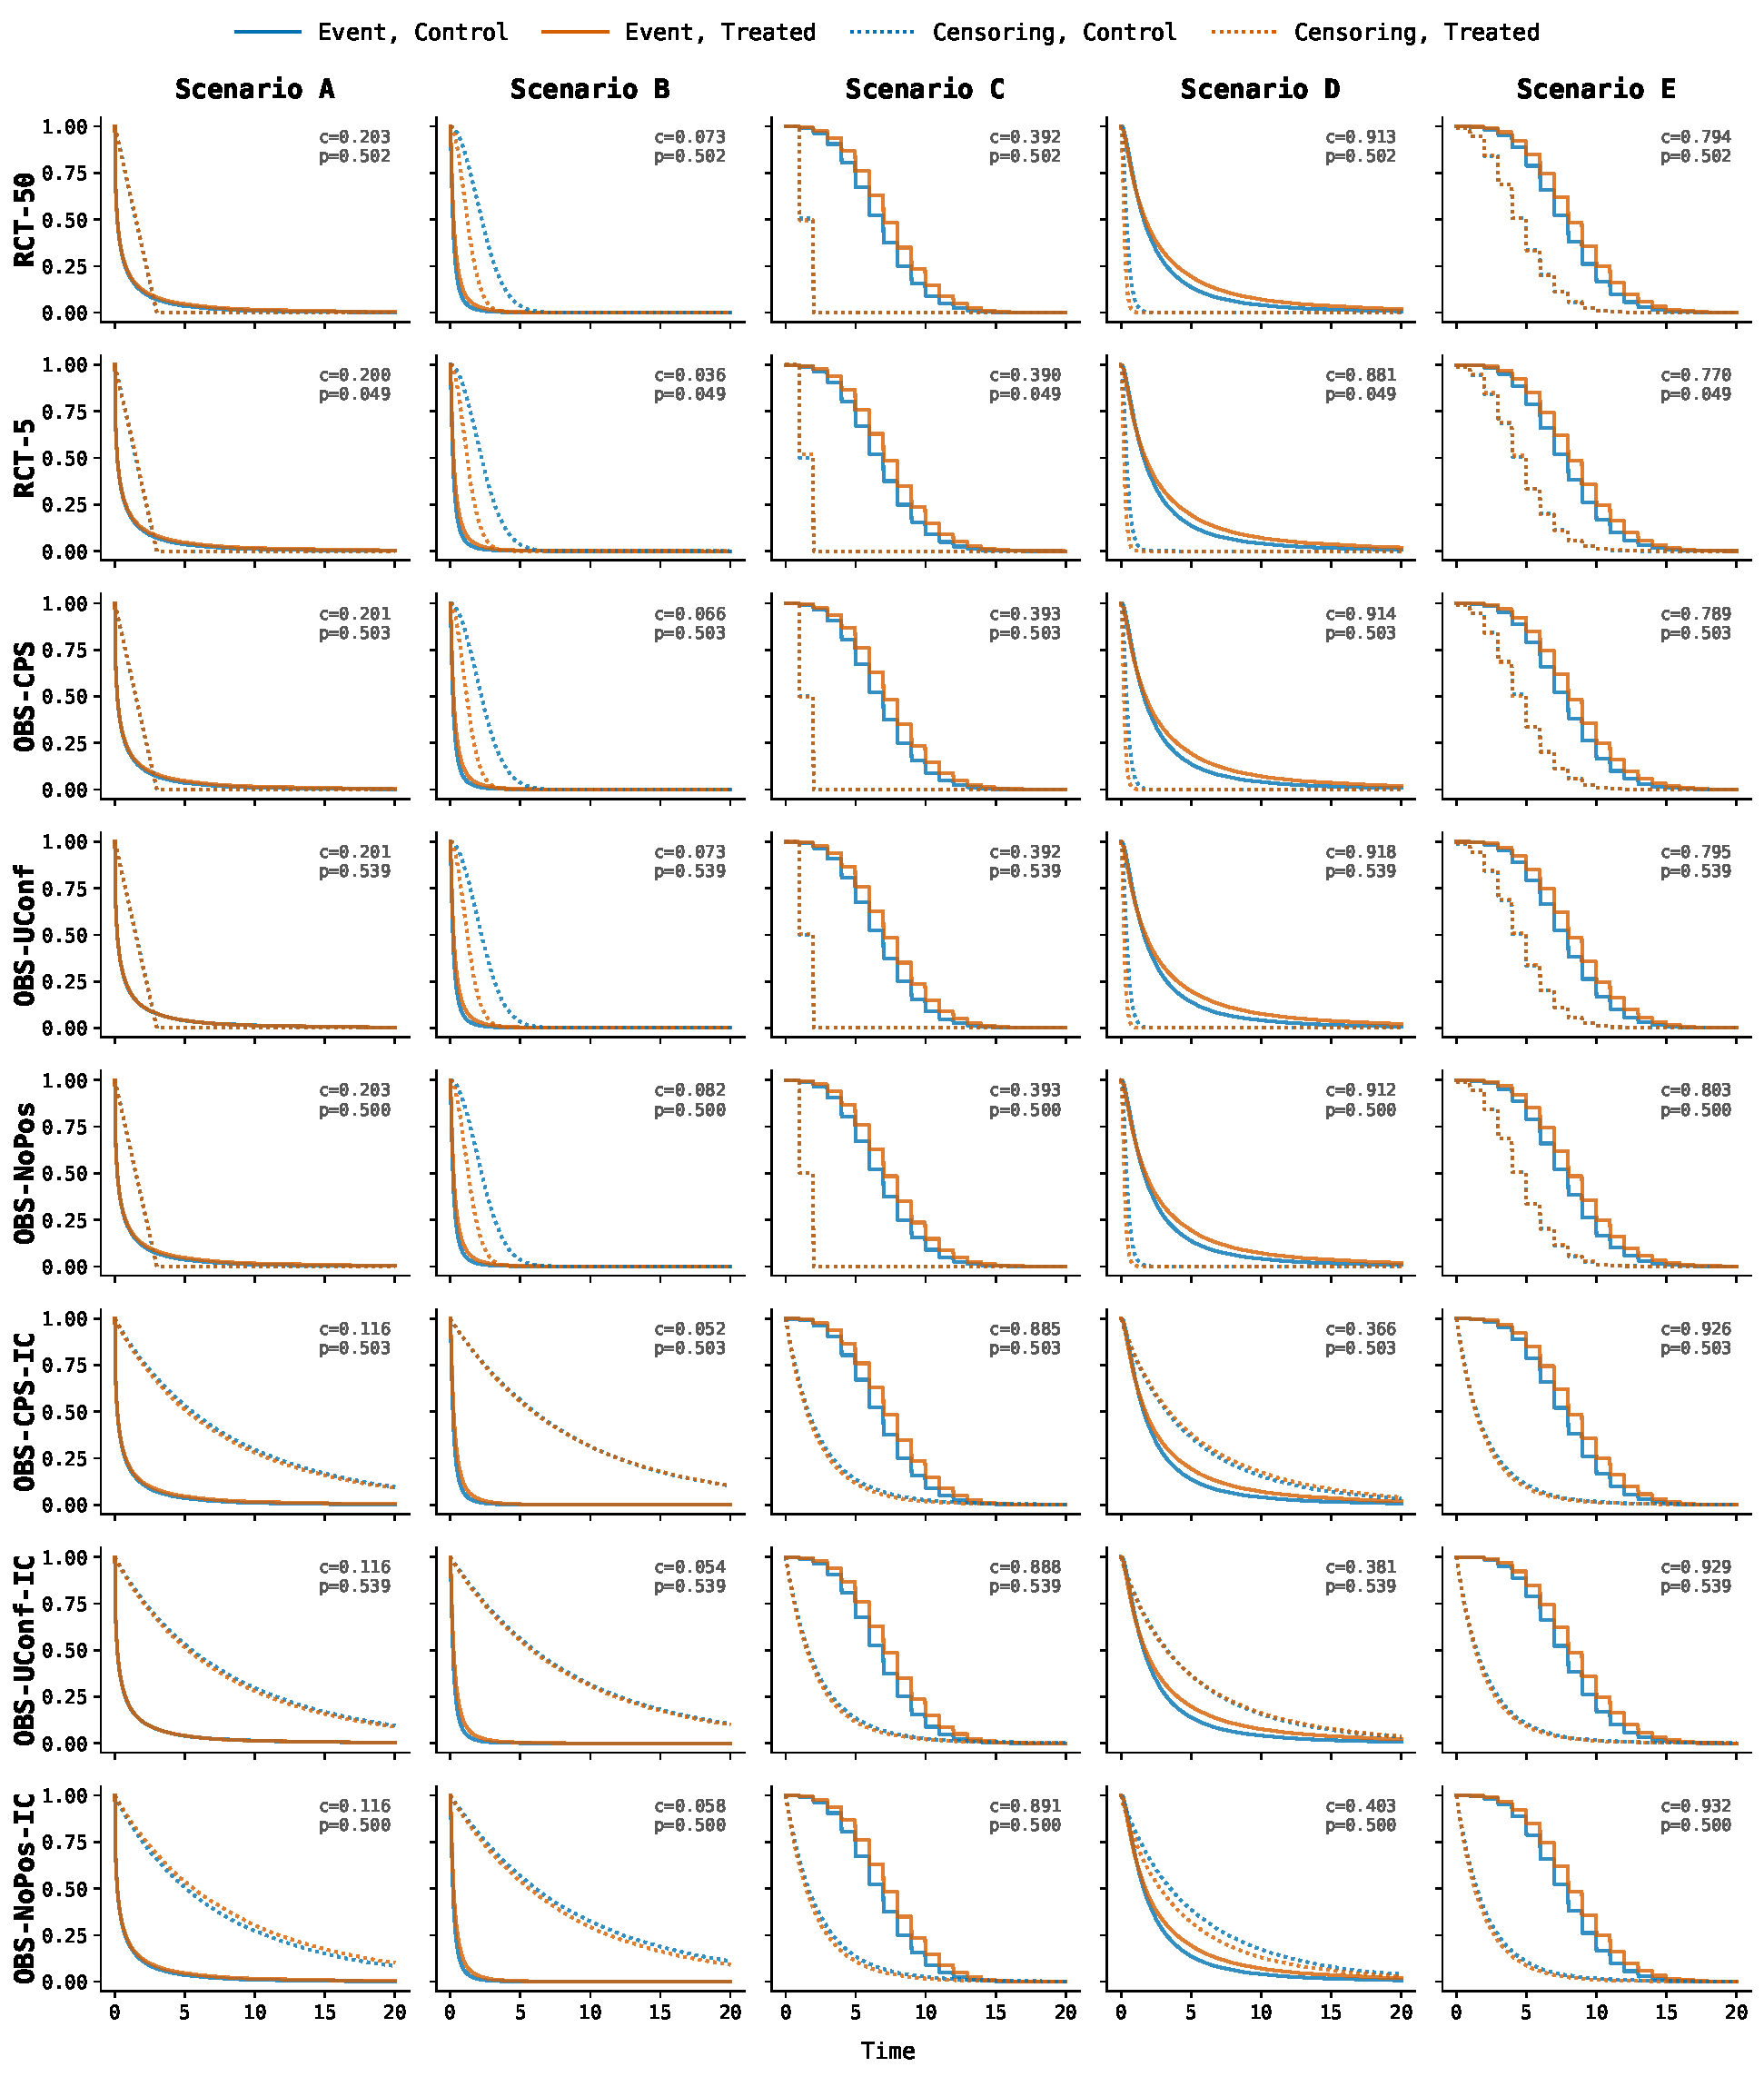
\includegraphics[width=1.0\linewidth]{Appendices/appendix-ch04/images/figure_results_updated/synthetic-km-curves.pdf} 
   
}
\end{figure}





\ChFourParagraph{\ChFourRebuttal{Remark on parameter calibration.}}
\ChFourRebuttal{The constants used in our synthetic generators are inherited from and aligned with prior causal-survival simulation setups~\citep{ch04:cui2023estimating,meir2025heterogeneous}, and are set to span distinct, interpretable regimes that the benchmark aims to cover. In particular, we calibrate (i) \emph{censoring severity} by shifting the relative scales of event-time and censoring-time processes (e.g., the AFT intercept change between Scenarios~\texttt{B} and~\texttt{D} increases typical event times and, together with the corresponding censoring model, yields higher censoring in \texttt{D}); (ii) \emph{treatment prevalence} and \emph{confounding strength} by adjusting propensity-score weights so that most configurations remain near balanced treatment except where imbalance is intentional (e.g., \texttt{RCT-5}), while allowing controlled dependence on observed or latent drivers; and (iii) \emph{effect magnitude/heterogeneity} through the coefficients on $W$ and $W$--covariate interactions, which we keep in a moderate range for comparability across scenarios. These choices are not unique, and alternative parameterizations could yield valid benchmarks; our goal is to provide a principled and reproducible instantiation that cleanly separates survival dynamics from causal-assumption stress and produces a broad range of survival CATE evaluation settings.}




